\section{Opgave 2 - Watch with six digits}
\begin{enumerate}
	\item[1)]
	
	Vi udvider koden ved hjælp af endnu en fil kaldet \verb|watch_ext|, hvor vi har følgende programmering:
	
	\begin{lstlisting}[caption={VHDL code for binary circular watch with 6 digits},label={lst:Watch6digits}]
	library ieee;
	use ieee.std_logic_1164.all;
	use ieee.numeric_std.all;
	
	entity watch_ext is
	port( clk, speed, reset : in std_logic;
	mode : in std_logic_vector(1 downto 0);
	seg1, seg10, seg100, seg1000, seg10000, seg100000 : out std_logic_vector(6 downto 0);
	cout : out std_logic;
	bin_val : out std_logic_vector(3 downto 0));
	end watch_ext;
	
	architecture timer of watch_ext is
	signal i_cout, i_cout1, i_cout10, i_cout100, i_cout1000, i_cout10000, reset_sig : std_logic; 
	signal bin_val_h1, bin_val_h10 : std_logic_vector(3 downto 0);
	
	begin
	c1: entity work.watch port map(clk => clk, reset => reset_sig, speed => speed, cout => i_cout);
	s1: entity work.counter port map(clk => i_cout, mode => "00", reset => reset_sig, seg => seg1, cout => i_cout1, bin_val => open);
	s10: entity work.counter port map(clk => i_cout1, mode => "01", reset => reset_sig, seg => seg10, cout => i_cout10, bin_val => open);
	m1: entity work.counter port map(clk => i_cout10, mode => "00", reset => reset_sig, seg => seg100, cout => i_cout100, bin_val => open);
	m10: entity work.counter port map(clk => i_cout100, mode => "01", reset => reset_sig, seg => seg1000, cout => i_cout1000, bin_val => open);
	h1: entity work.counter port map(clk => i_cout1000, mode => "00", reset => reset_sig, seg => seg10000, cout => i_cout10000, bin_val => bin_val_h1);
	h10: entity work.counter port map(clk => i_cout10000, mode => "11", reset => reset_sig, seg => seg100000, cout => open, bin_val => bin_val_h10);
	
	process (bin_val_h1, bin_val_h10)
	
	begin
	reset_sig <= '1';
	if reset = '0' then
	reset_sig <= '0';
	elsif bin_val_h1 = "0100" and bin_val_h10 = "0010" then
	reset_sig <= '0';
	end if;
	end process;
	
	end timer;
	
	\end{lstlisting}
	
	\item[2)] Vi tester vores watch på DE2-boardet. På følgende billeder kan forskellige værdier klokkeslæt ses:
	\begin{figure}[h]
		\centering
		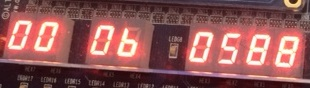
\includegraphics[scale=0.9]{pictures/Oevelse6/opg2/6min.JPG}
		\caption{klokkeslæt på uret inkl minutter og sek}
		\label{fig:alarm0}
		\end{figure}
	\begin{figure}[h]
		\centering
		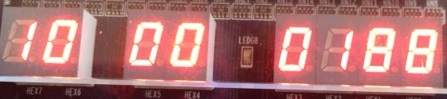
\includegraphics[scale=0.8]{pictures/Oevelse6/opg2/10timer.JPG}
		\caption{Klokkeslæt inkl timer, minutter og sek}
		\label{fig:alarm0}
	\end{figure}
	\begin{figure}[h]
		\centering
		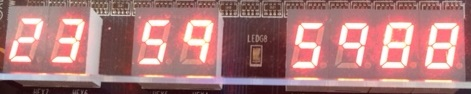
\includegraphics[scale=0.8]{pictures/Oevelse6/opg2/upper_limit.JPG}
		\caption{Øverste grænse inden uret resetter sig til 00.00.00}
		\label{fig:alarm0}
	\end{figure}
\end{enumerate}